\section{Production}

The production of the position-sensitive device involves the necessary steps to produce the detector and arithmetic \gls{pcb}.

It's best to first do the arithmetic board and if it works, proceed with the detector.
Of course, if you only need one of the boards, perform the following steps only once.

\subsection{Commissioning}

% TODO: screenshots of HTML BOM files

Before we can assemble the \gls{pcb}s, we need to gather the required components and order missing pieces.

The list of the required components is usually known as the \gls{bom}.
You can generate a current \gls{bom} directly from \href{https://kicad-pcb.org}{KiCad} by using the \href{https://github.com/openscopeproject/InteractiveHtmlBom}{InteractiveHtmlBom} plugin.
The plugin generates an \gls{html} file that lists the components and their respective placement on the \gls{pcb}.
\Cref{fig:kicad_interactive_html_bom_plugin_menu} shows where to find the plugin in the \gls{pcb} editor menu.
You can check if the parts are stocked and placed.
\begin{figure}[H]
	\centering
	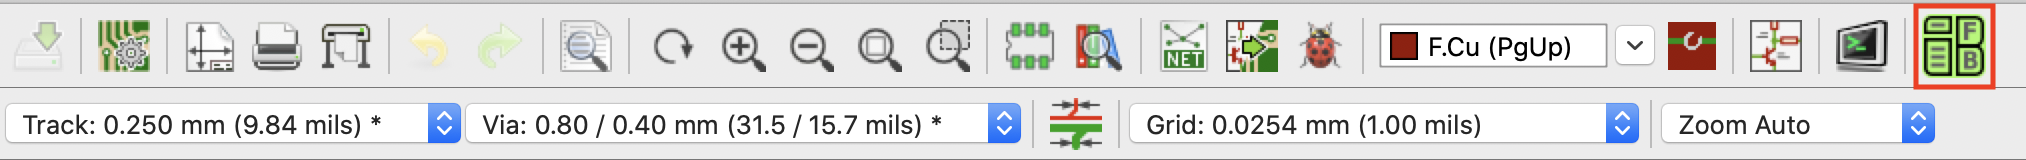
\includegraphics[scale=0.4]{screenshot/kicad_interactive_html_bom_plugin_menu}
	\caption{Menu entry for the \href{https://github.com/openscopeproject/InteractiveHtmlBom}{InteraciveHtmlBom} plugin for \href{https://kicad-pcb.org}{KiCad}}\label{fig:kicad_interactive_html_bom_plugin_menu}
\end{figure}
\Cref{fig:kicad_interactive_html_bom_plugin_arithmetic} and \cref{fig:kicad_interactive_html_bom_plugin_detector} show the view of the generated \gls{html} for the arithmetic and detector board.
\begin{figure}[H]
	\centering
	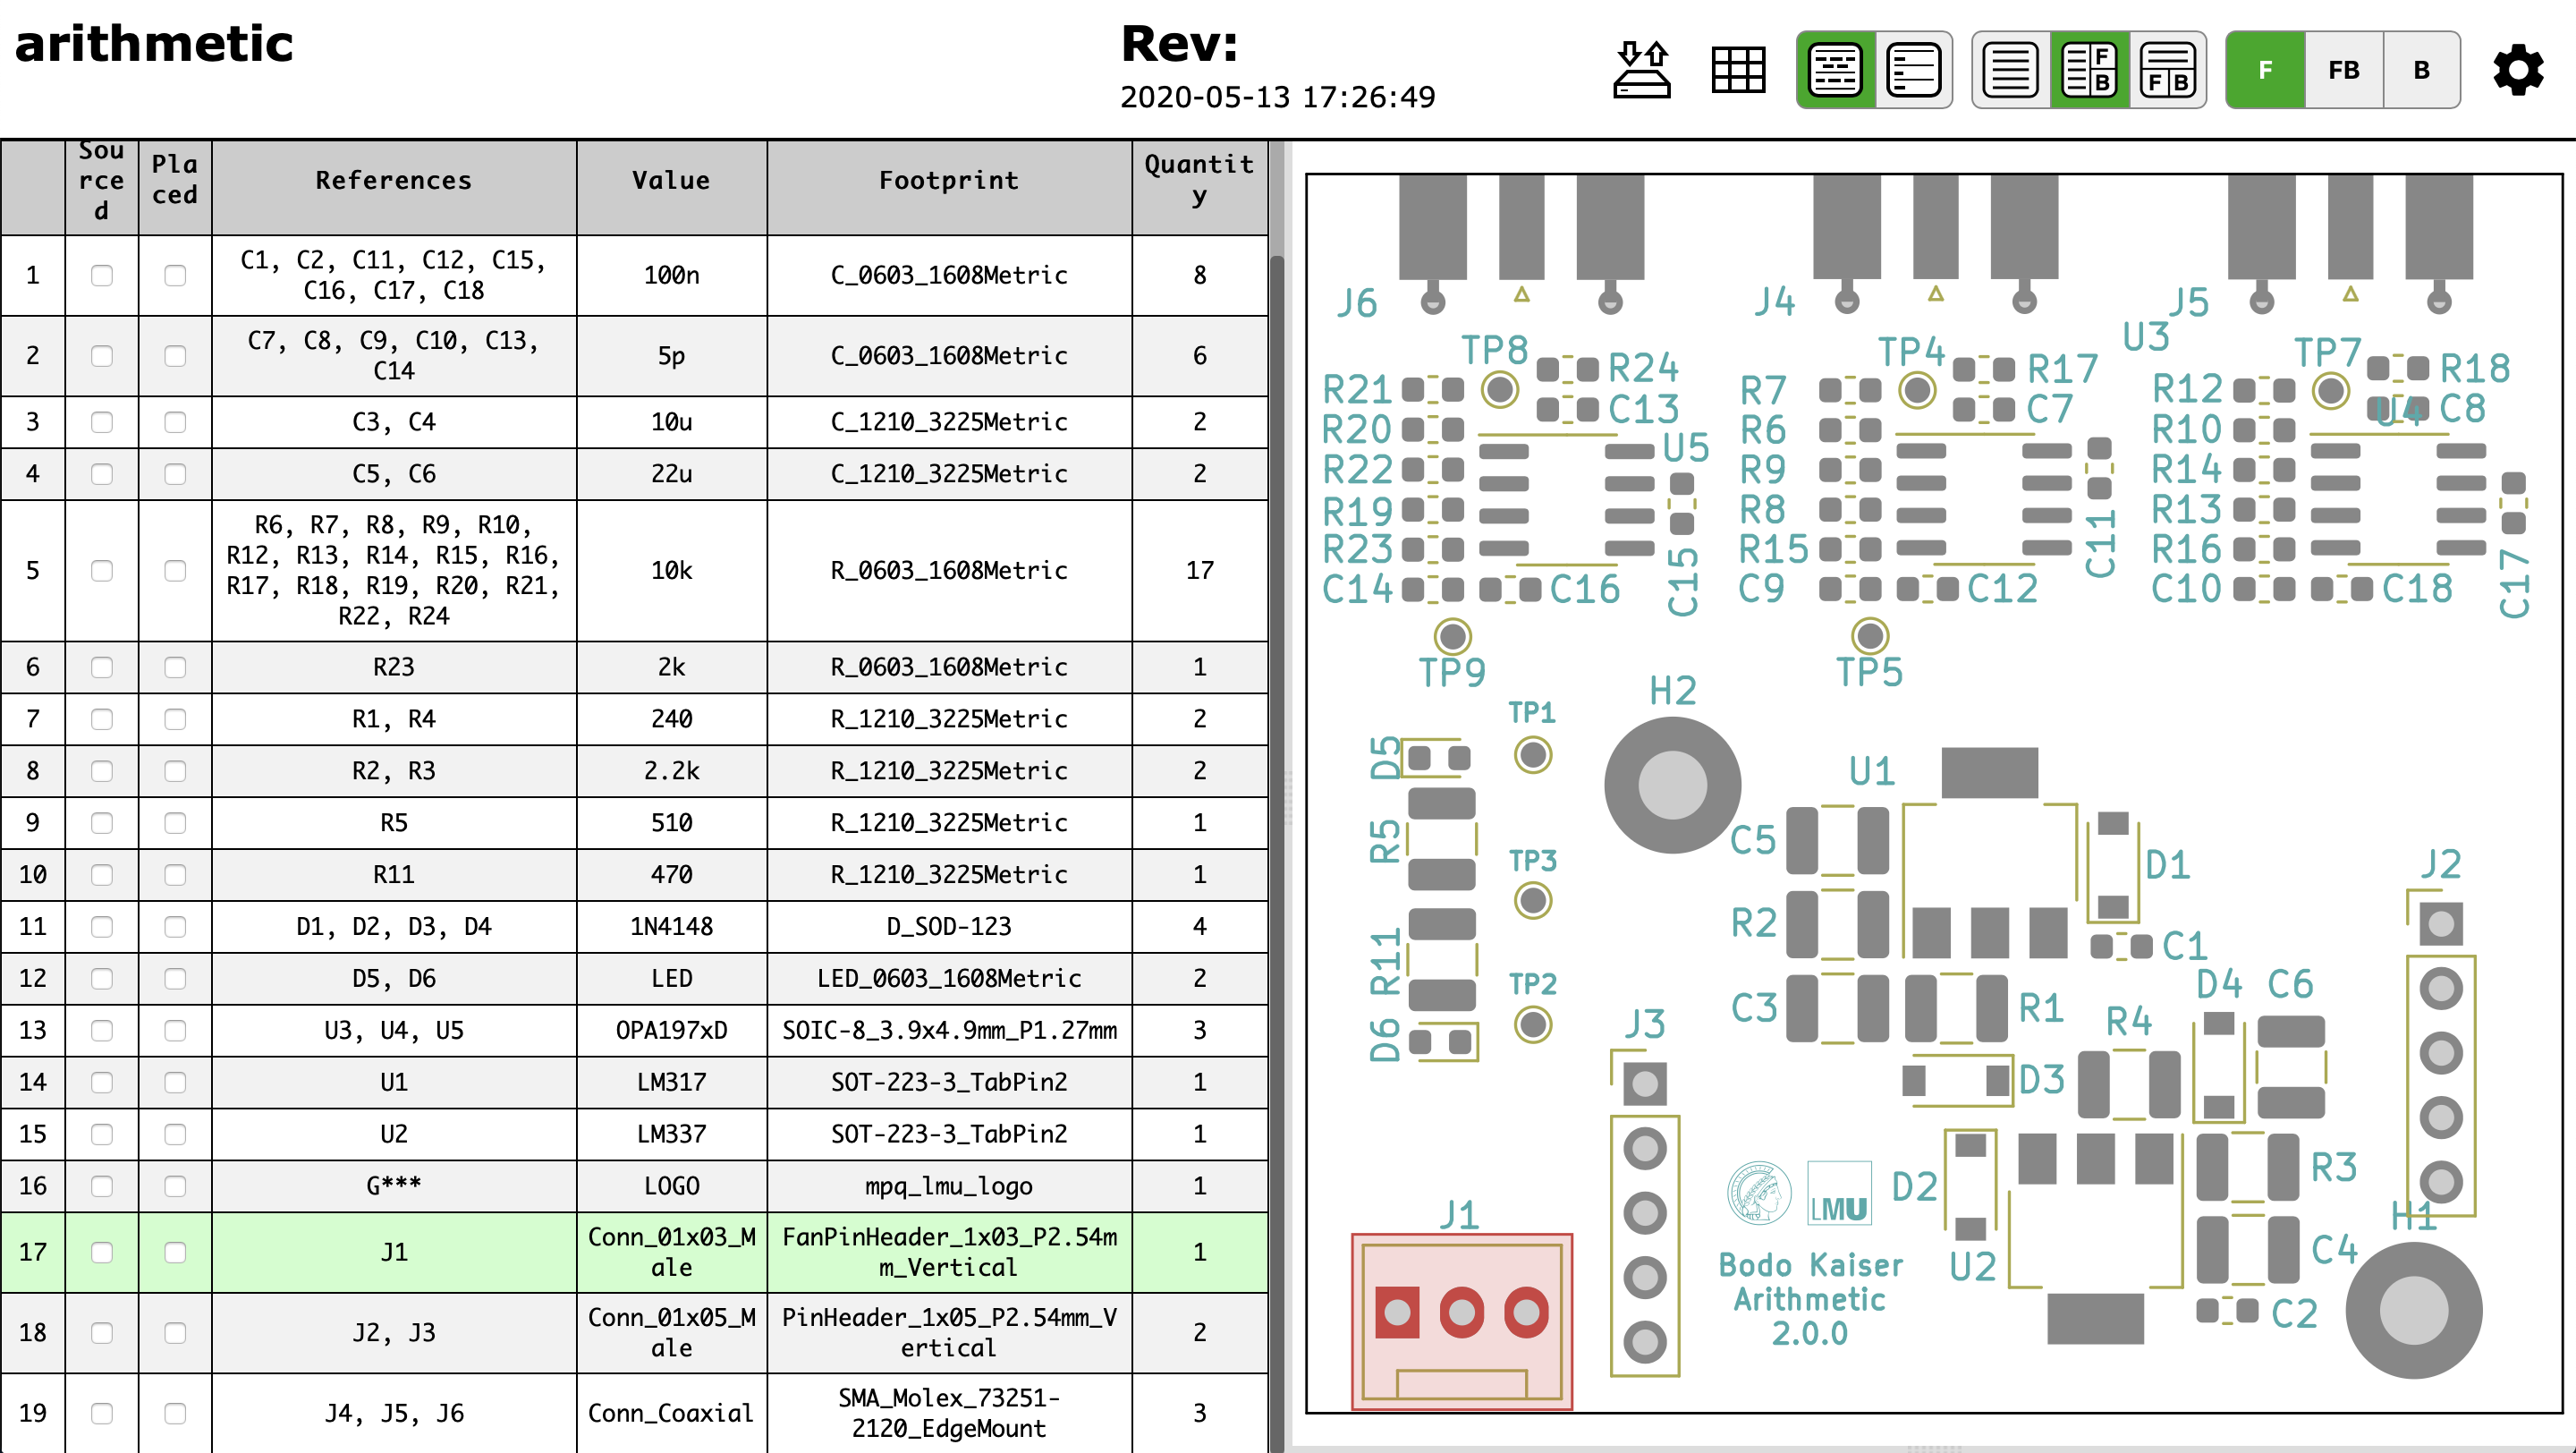
\includegraphics[scale=0.3]{screenshot/kicad_interactive_html_bom_plugin_arithmetic}
	\caption{Arithmetic board view of the \href{https://github.com/openscopeproject/InteractiveHtmlBom}{InteraciveHtmlBom} plugin}\label{fig:kicad_interactive_html_bom_plugin_arithmetic}
\end{figure}
\begin{figure}[H]
	\centering
	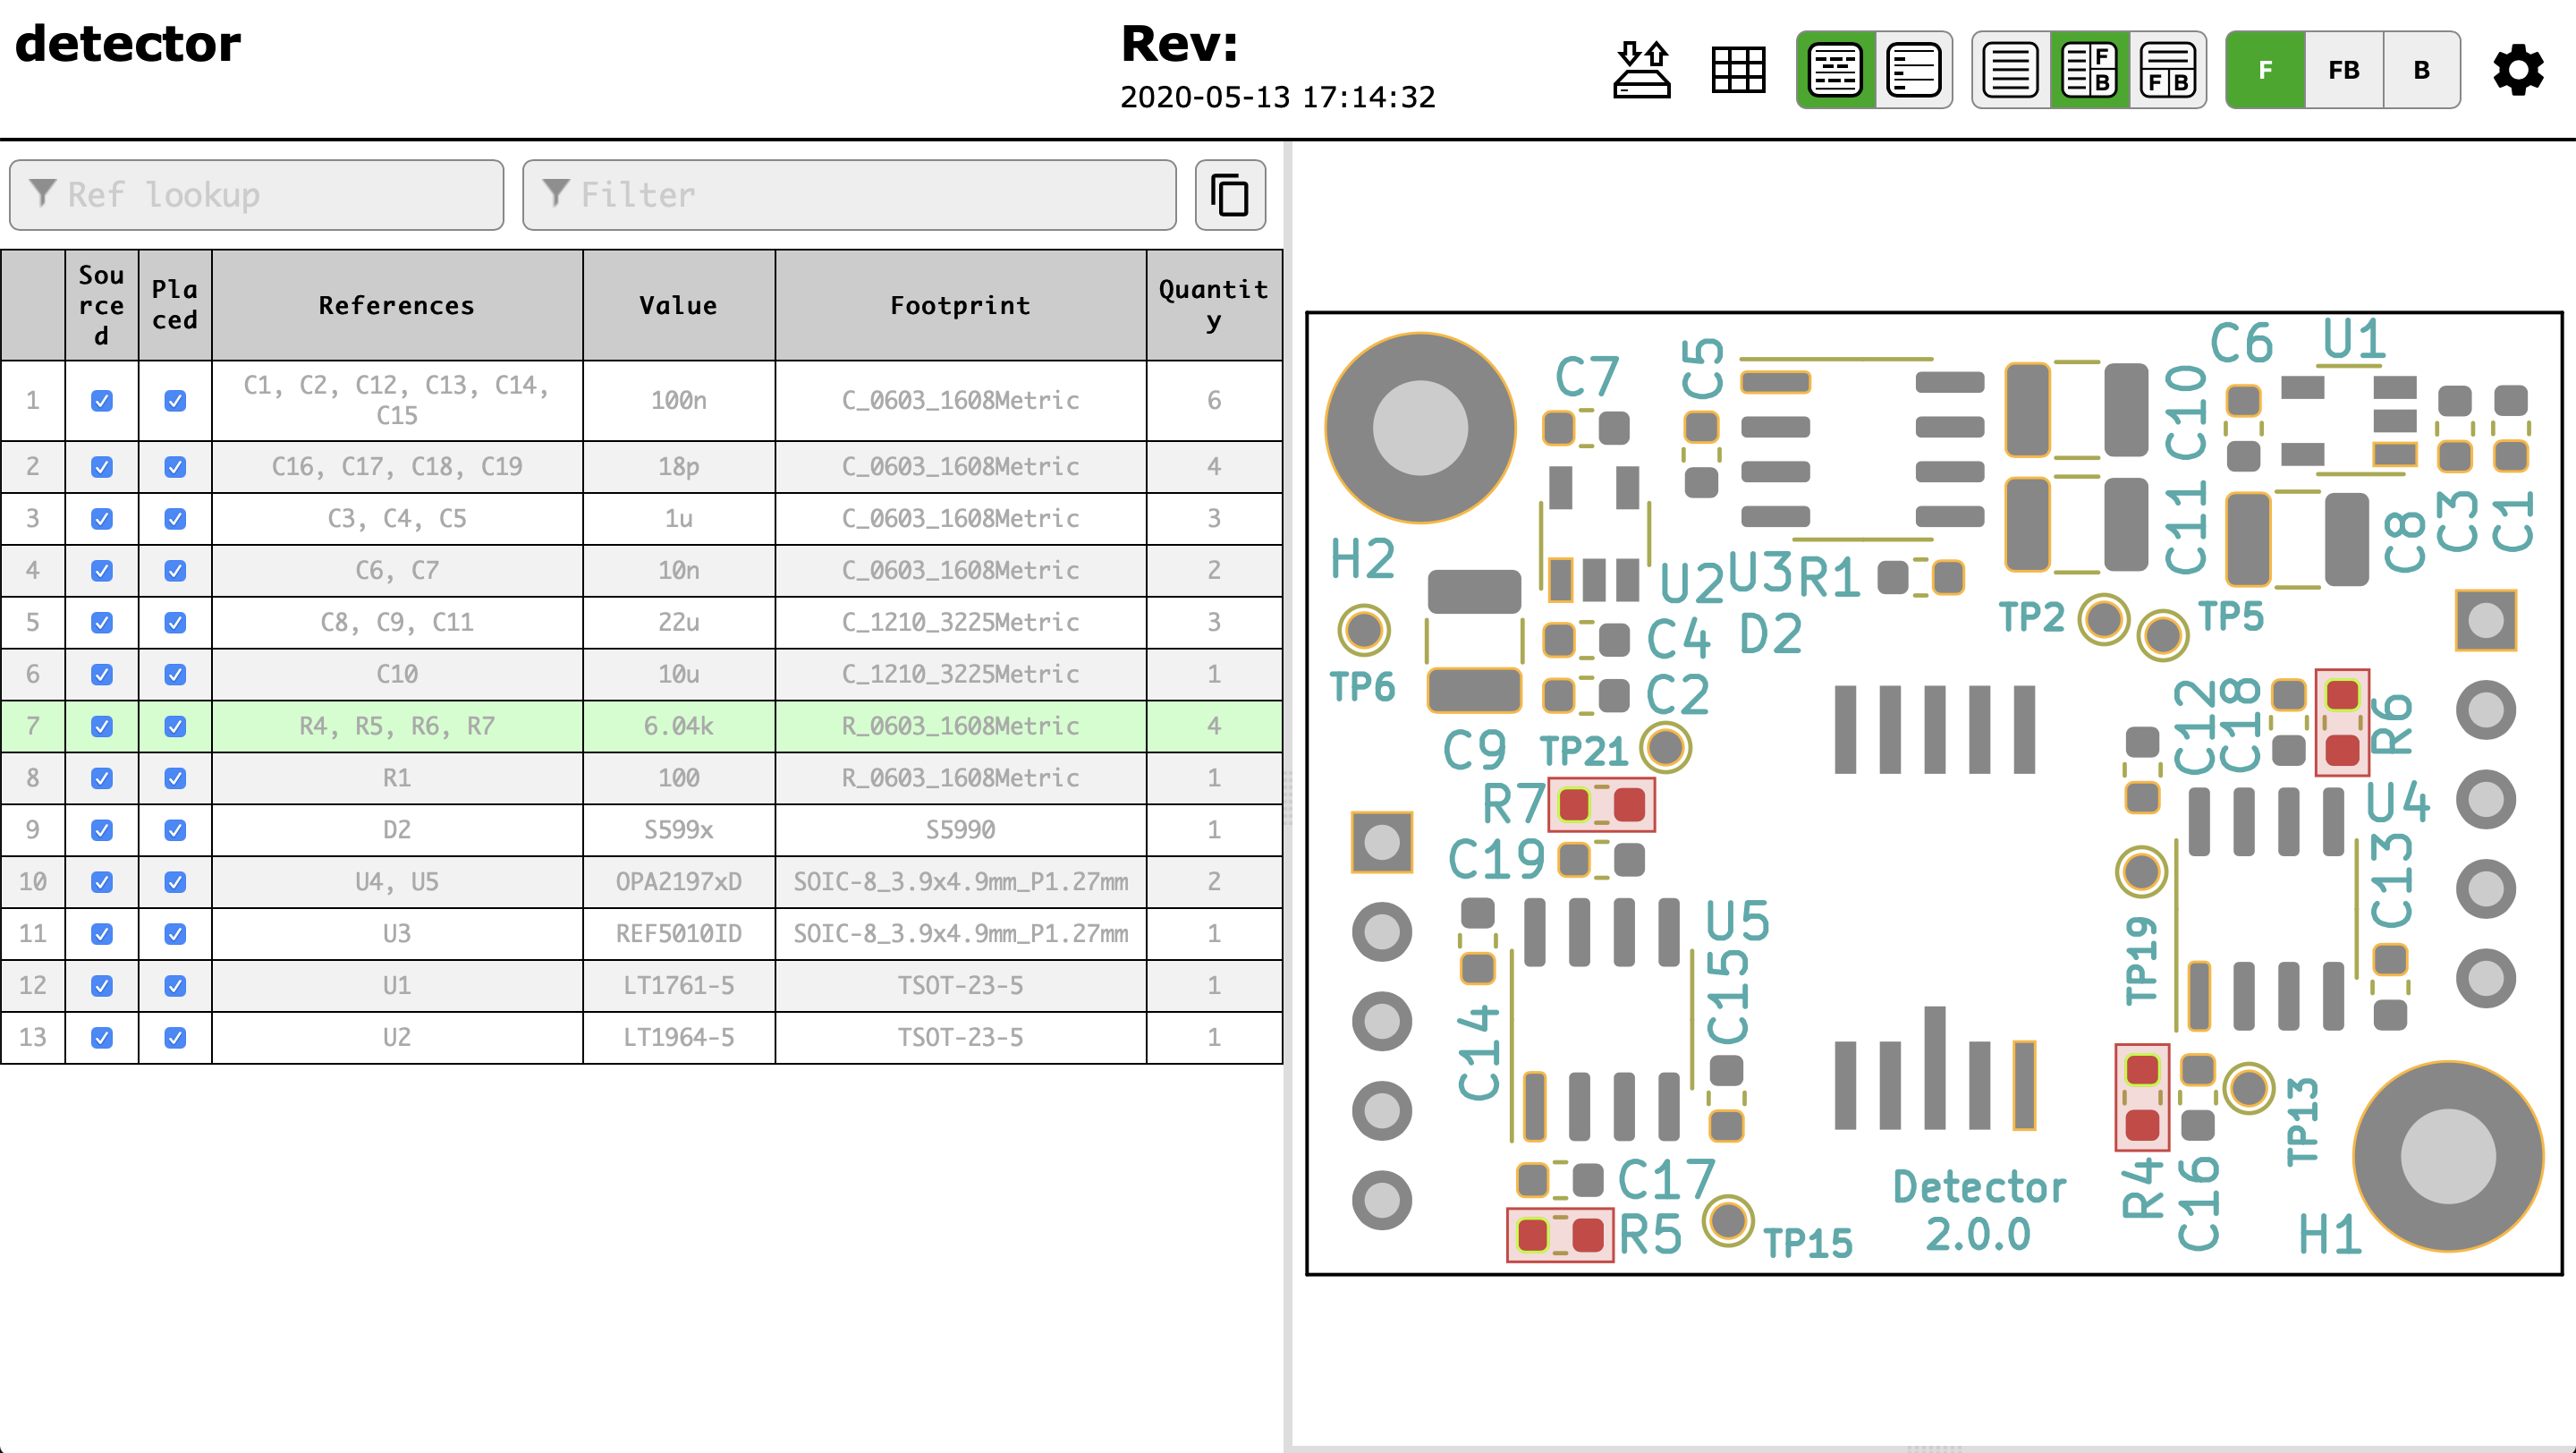
\includegraphics[scale=0.3]{screenshot/kicad_interactive_html_bom_plugin_detector}
	\caption{Detector board view of the \href{https://github.com/openscopeproject/InteractiveHtmlBom}{InteraciveHtmlBom} plugin}\label{fig:kicad_interactive_html_bom_plugin_detector}
\end{figure}
Start by checking the local inventory for the components listed by the generated \gls{html} \gls{bom}.
If certain elements are missing, you can check the \path{BOM.xlsx} file inside the project repository.
It contains part numbers and product links from major electronic distributors.
If you order, double-check with the generated \gls{html} \gls{bom}.
There might be errors, e.g., wrong casing sizes in the \path{BOM.xlsx} as it is potentially outdated.

\subsection{Manufacturing}

After you sourced the components, you can place them using the solder paste on the PCB.

Put on rubber gloves as the solder paste is potentially hazardous. Take out the solder paste from the fridge and let it reach room temperature. It is possible to use the cold solder paste directly, but it makes the handling more difficult as the paste is less fluid.

Place the solder paste onto the contacts of the PCB. Generally speaking, it is better to have too much solder paste then too less. If there is a small overlap between the contacts, this is fine as the solder will shrink when transitioning to a liquid phase in the oven.

Now, place the SMD components onto the solder with a tweezer. For me, it works best to start with the larger components and then progress to the smaller ones. You can check the components as placed in the generated HTML BOM.

%\subsection{Reflow soldering}

Start the oven and adjust the frame on which you place the board with the screw to the appropriate size. Use an empty PCB for this.
After that, select the profile SMD180 and follow the instructions of the oven.

\subsection{Quality control}

Inspect the board for misplaced components and unmelted solder. You can use the solder heat gun to melt the remaining solder paste or remove misplaced components. However, you might blow away small capacitors.
You can fix other defects by hand soldering.

% \subsection{Hand soldering}

Some components, for example, the SMA mounts or the pin headers, have to be soldered by hand. Before soldering these components by hand, jump to the electrical testing section. Only, if your board passes the electrical tests, proceed with hand soldering the missing parts.

\subsection{Electrical testing}

With the electrical testing, we want to confirm that the solder connections and components work as expected.
The most basic check is that the supply voltages are correct.
More elaborated checks concern the operational amplifiers but are out of the scope of this document.

% \subsubsection{Arithmetic board I}

Leave the arithmetic board unpowered and measure the resistance between the supply lines through the test points TP1 (+12 V), TP2 (GND), and TP3 (-12 V).
There should be very high resistance between any of these test points.
Otherwise, there is a short.

If no short is detected, you can configure the power supply to provide a dual voltage of +- 15 V.
Alternatively, use two single voltage sources set to 15 V and connect the negative port of one of the voltage sources with the other one's positive voltage.
Confirm that the output voltages are correct with the multimeter. If possible, limit the current of the voltage sources.
You can set the current limit as low as possible and increase from there until the voltage becomes stable.
You might need to adjust the limit when connecting the voltages with the arithmetic board.

Connect the power supply with the arithmetic board but double-check the polarity.
The voltage between TP2 (GND) and TP1 (+12 V) should read around + 12 V while the voltage between TP2 (GND) and TP3 (- 12 V) should read about - 12 V.

Confirm that the supply voltages reach the op-amps.
Check the temperature of the op-amps.
If the op-amps are very hot, there is a short.
You can additionally check if the op-amps work by grounding the inverting input.
Because the op-amp's non-inverting input is connected with the ground, the op-amp output should be a virtual ground.

% \subsubsection{Detector board}

Have the detector board unplugged and measure the resistance between GND (you can use the center pin of the headers), TP5 (+ 5V), and TP6 (-5 V). If the resistance is high, proceed. Otherwise, find the short.

Measure the voltage between the photodiode and GND's outer pins while illuminating the sensitive area of the photodiode with a laser pointer.
You should detect a small voltage.

If the preceding checks are successful, mount the detector board on the arithmetic board, and measure the detector board's supply voltages.

Finally, confirm that the voltage reference (U3) outputs 10 V and that the op-amps have the correct supply voltage.

% \subsubsection{Arithmetic board II}

Leave the detector board mounted on the arithmetic board.
Measure the voltage at the outputs of the operational amplifiers of the arithmetic board.
For the summing amplifier (U5), we expect an increase in voltage when illuminating the photodiode with the laser pointer.
For the difference amplifiers (U3, U4), we expect the voltage to change when moving the laser pointer's focal spot on the photodiode.

